Während bei dem Meilensteinplan nur die Meilensteine abgebildet sind, werden im Projektbalkenplan alle Arbeitspakete und deren ungefähres Fälligkeitsdatum gezeigt. So hat man jederzeit einen Überblick über den terminlichen Status des Projektfortschritts. Daher ist der Projektbalkenplan oder \enquote{Gantt-Chart}  als zeitliche Ebene die erste Wahl, um einen umfassenden Überblick über den zeitlichen Status des Projektfortschritts zu behalten \cite[vgl.][]{domendos:2019}. \\
Auf der nächsten Seite befindet sich mit Abbildung \ref{fig:projektbalkenplan} der Balkenplan, der nach dem \enquote{PSP} aufgebaut ist.

\begin{landscape}
	\begin{figure}[H]
		\centering
		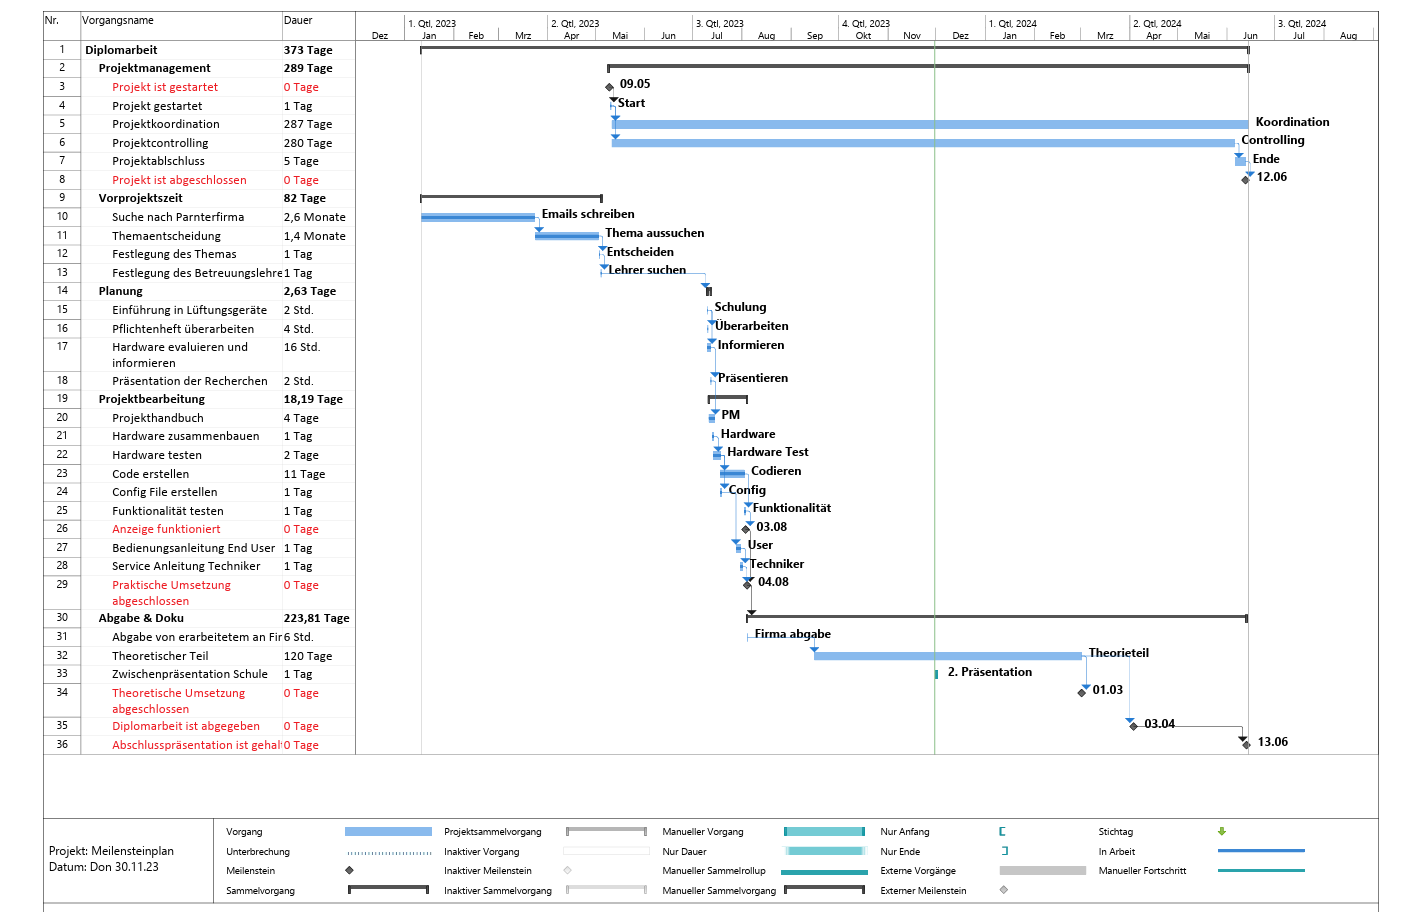
\includegraphics[width=0.9\linewidth]{Bilder/ganttchart}
		\caption{Projektbalkenplan}
		\label{fig:projektbalkenplan}
	\end{figure}
\end{landscape}